\documentclass[12pt,a4paper]{article}

\usepackage[utf8]{inputenc}
\usepackage[T1]{fontenc}
\usepackage{mathpazo}
\usepackage[margin=1.15in]{geometry}
\usepackage{setspace}
\usepackage{hyperref}
\usepackage{titlesec}
\usepackage{amsmath,amsthm,amssymb}
\usepackage{booktabs}
\usepackage{enumitem}
\usepackage{fancyhdr}
\usepackage{xcolor}
\usepackage{tcolorbox}
\usepackage{tikz}
\usepackage{array}
\usepackage{float}

\hypersetup{colorlinks=true, linkcolor=blue!70!black, citecolor=black, urlcolor=blue!70!black}

\titleformat{\section}{\large\bfseries}{\thesection}{0.7em}{}
\titleformat{\subsection}{\normalsize\bfseries}{\thesubsection}{0.7em}{}
\titleformat{\subsubsection}{\normalsize\itshape}{\thesubsubsection}{0.7em}{}

\newtheorem{definition}{Definition}[section]
\newtheorem{proposition}[definition]{Proposition}
\newtheorem{theorem}[definition]{Theorem}
\newtheorem{lemma}[definition]{Lemma}
\newtheorem{corollary}[definition]{Corollary}
\newtheorem{example}[definition]{Example}
\theoremstyle{remark}
\newtheorem{remark}[definition]{Remark}

\newcommand{\R}{\mathbb{R}}
\newcommand{\ones}{\mathbf{1}}
\newcommand{\x}{\mathbf{x}}
\newcommand{\bb}{\mathbf{b}}
\DeclareMathOperator*{\argmax}{arg\,max}
\DeclareMathOperator{\Var}{Var}
\DeclareMathOperator{\Cov}{Cov}

\newtcolorbox{intuition}[1][]{colback=blue!3, colframe=blue!40!black,
  fonttitle=\bfseries, title={Intuition: #1}, sharp corners, boxrule=0.5pt}
\newtcolorbox{keyinsight}[1][]{colback=orange!5, colframe=orange!60!black,
  fonttitle=\bfseries, title={Key Structural Insight}, sharp corners, boxrule=0.5pt}
\newtcolorbox{prebisch}[1][]{colback=green!3, colframe=green!40!black,
  fonttitle=\bfseries, title={Prebisch Connection: #1}, sharp corners, boxrule=0.5pt}
\newtcolorbox{vizpanel}[1][]{colback=gray!4, colframe=gray!50!black,
  fonttitle=\bfseries, title={Visualization: #1}, sharp corners, boxrule=0.5pt}

\setlength{\parindent}{1.5em}
\onehalfspacing
\setlength{\headheight}{14pt}
\pagestyle{fancy}
\fancyhf{}
\fancyhead[L]{\small\itshape Chapter 10: The Formal Formation Model}
\fancyhead[R]{\small\thepage}
\renewcommand{\headrulewidth}{0.4pt}

\title{\vspace{-1cm}\textbf{Chapter 10} \\[0.5em]
\LARGE The Formal Formation Model \\[0.3em]
\large\textit{The Complete Dynamic System}}
\author{}
\date{}

\begin{document}
\maketitle
\thispagestyle{fancy}

\begin{quote}
\textit{``As situa\c{c}\~{o}es de depend\^{e}ncia na Am\'{e}rica Latina contempor\^{a}nea sup\~{o}em um modo de articula\c{c}\~{a}o entre a din\^{a}mica econ\^{o}mica e a a\c{c}\~{a}o social que \'{e} distinto tanto da expans\~{a}o dos centros como daquela dos pa\'{i}ses coloniais.''}\\[0.3em]
\textnormal{[``The situations of dependence in contemporary Latin America presuppose a mode of articulation between economic dynamics and social action that is distinct both from the expansion of the centers and from that of the colonial countries.'']}\\
\hfill --- Fernando Henrique Cardoso and Enzo Faletto, \textit{Depend\^{e}ncia e Desenvolvimento na Am\'{e}rica Latina} (1969)
\end{quote}

\vspace{1em}

Chapter~9 introduced the formation equation: preferences evolve through $W^I$. Chapter~7 derived the bargaining equilibrium: allocations depend on power $\boldsymbol{\pi}(W)$ and preferences $\boldsymbol{\theta}$. This chapter closes the loop.

The formation model is a dynamical system with three equations:
\begin{enumerate}
\item The bargaining equilibrium determines allocations given power and preferences.
\item The return function maps allocations into observable outcomes.
\item The formation equation maps observed returns into next-period preferences.
\end{enumerate}

The loop $\boldsymbol{\theta}_t \to \x^*_t \to \mathbf{r}_t \to \boldsymbol{\theta}_{t+1}$ is the complete model. The steady state $(\boldsymbol{\theta}^*, \x^*, \mathbf{r}^*)$ is a fixed point of this system. Multiple fixed points can coexist in the same economy with the same $W$. Which one obtains depends on history --- on the initial $\boldsymbol{\theta}_0$, which was formed under a possibly different $W^I$.

This is the chapter that makes the book's title operational. An economy is not just a weight matrix $W$. It is a weight matrix, a preference vector formed by that matrix, and an allocation produced by the two together. Structure is not a constraint \textit{on} agents with given preferences. Structure is the process that \textit{produces} the preferences.


%% =====================================================================
\section{The Complete System}
\label{sec:system}
%% =====================================================================

\subsection{Three Equations}

\begin{definition}[The Formation Model]\label{def:model}
The \textbf{formation model} consists of three components operating in sequence within each generation $t$:

\textbf{Equation 1: The Bargaining Equilibrium.} Given power $\boldsymbol{\pi}(W)$, preferences $\boldsymbol{\theta}_t$, and endowments $\boldsymbol{\omega}$:
\begin{equation}\label{eq:bargaining}
x_{i,t}^* = h(\pi_i, \theta_{i,t}, \omega_i) = \frac{\Omega}{N} + \frac{1}{\kappa}\left(\pi_i - \frac{1}{N}\right) + \frac{\theta_{i,t} - \bar{\theta}_t}{N\kappa}\Phi,
\end{equation}
where $\bar{\theta}_t = \frac{1}{N}\sum_j \theta_{j,t}$ and $\Phi > 0$ is a scaling factor. The first correction is from power (Chapter~7); the second is from preference heterogeneity. An agent who is more patient/ambitious than average ($\theta_{i,t} > \bar{\theta}_t$) invests more and consumes less in the current period.

\textbf{Equation 2: The Return Function.} The allocation produces observable returns:
\begin{equation}\label{eq:returns}
r_{i,t} = g_i(x_{i,t}^*, \x_{-i,t}^*) = \alpha_i + \beta_i x_{i,t}^* + \gamma_i \sum_j W^P_{ij} x_{j,t}^*,
\end{equation}
where $\alpha_i$ is a sector-specific baseline, $\beta_i$ is the private return to investment, and $\gamma_i \sum_j W^P_{ij} x_{j,t}^*$ is the network spillover: your return depends on what your production neighbors invest. This is the Leontief amplifier from Chapter~3.

\textbf{Equation 3: The Formation Equation.} Observed returns update preferences for the next generation:
\begin{equation}\label{eq:formation}
\theta_{i,t+1} = \rho\theta_{i,t} + (1-\rho)\bar{\theta}_0 + \mu\left(\sum_j W^I_{ij} r_{j,t} - r^*\right).
\end{equation}
\end{definition}

The three equations form a map $\Phi: \R^N_+ \to \R^N_+$:
\begin{equation}\label{eq:map}
\boldsymbol{\theta}_{t+1} = \Phi(\boldsymbol{\theta}_t) \equiv \rho\boldsymbol{\theta}_t + (1-\rho)\bar{\theta}_0\ones + \mu\left(W^I \mathbf{g}(\mathbf{h}(\boldsymbol{\pi}, \boldsymbol{\theta}_t, \boldsymbol{\omega})) - r^*\ones\right).
\end{equation}

This is a nonlinear dynamical system in $\boldsymbol{\theta}$. The weight matrices $(W, W^P, W^I)$ and parameters $(\rho, \mu, \bar{\theta}_0, r^*, \kappa, \boldsymbol{\alpha}, \boldsymbol{\beta}, \boldsymbol{\gamma})$ are structural. The dynamics are in $\boldsymbol{\theta}$.

\begin{intuition}[The loop in words]
\textbf{Generation $t$}: You arrive with preferences $\theta_{i,t}$ inherited from your parents' generation and your own early-life signals. Given those preferences and your structural power $\pi_i$, the bargaining equilibrium determines your allocation $x_{i,t}^*$. Your allocation, combined with the production network, produces your return $r_{i,t}$. Your children observe your return (and your neighbors' returns, weighted by $W^I$). They form preferences $\theta_{i,t+1}$ based on what they saw. They enter the next generation's bargaining equilibrium. The loop continues.

\textbf{The standard model} runs this loop once (at $t = 0$, with $\boldsymbol{\theta}_0$ given) and stops. The formation model runs it forever.
\end{intuition}


\subsection{The Linearized System}

For analysis, linearize around a candidate steady state $\boldsymbol{\theta}^*$. Let $\boldsymbol{\delta}_t = \boldsymbol{\theta}_t - \boldsymbol{\theta}^*$. The Jacobian of the map $\Phi$ at $\boldsymbol{\theta}^*$:

\begin{equation}\label{eq:jacobian}
J = D\Phi(\boldsymbol{\theta}^*) = \rho I + \mu W^I G' H',
\end{equation}
where $G' = \text{diag}(\partial g_i / \partial x_i) + \gamma W^P$ is the Jacobian of the return function (incorporating network spillovers) and $H' = \text{diag}(\partial h_i / \partial \theta_i)$ is the Jacobian of the bargaining equilibrium with respect to preferences.

\begin{proposition}[Structure of the Jacobian]\label{prop:jacobian}
The Jacobian $J$ has three components:
\begin{equation}\label{eq:J_decomp}
J = \underbrace{\rho I}_{\text{persistence}} + \underbrace{\mu \beta_{\text{eff}} \cdot W^I \cdot \text{diag}(H')}_{\text{direct formation}} + \underbrace{\mu \gamma_{\text{eff}} \cdot W^I W^P \cdot \text{diag}(H')}_{\text{network-amplified formation}},
\end{equation}
where $\beta_{\text{eff}}$ and $\gamma_{\text{eff}}$ are effective return parameters.

The spectral radius of $J$ determines stability: $\rho(J) < 1$ implies the steady state is stable. The eigenvalues of $J$ combine the eigenvalues of $W^I$, $W^P$, and the persistence $\rho$ in a nontrivial way.
\end{proposition}


%% =====================================================================
\section{Steady States}
\label{sec:steady}
%% =====================================================================

\subsection{Existence and Characterization}

A steady state is a fixed point $\boldsymbol{\theta}^* = \Phi(\boldsymbol{\theta}^*)$. From~\eqref{eq:map}:
\begin{equation}\label{eq:steady_state}
(1 - \rho)(\boldsymbol{\theta}^* - \bar{\theta}_0\ones) = \mu\left(W^I\mathbf{g}(\mathbf{h}(\boldsymbol{\pi}, \boldsymbol{\theta}^*, \boldsymbol{\omega})) - r^*\ones\right).
\end{equation}

Agent by agent:
\begin{equation}\label{eq:steady_i}
\theta_i^* = \bar{\theta}_0 + \frac{\mu}{1-\rho}\left(\sum_j W^I_{ij} g_j(h_j(\pi_j, \theta_j^*, \omega_j)) - r^*\right).
\end{equation}

The steady-state preference deviates from the anchor by $\frac{\mu}{1-\rho}$ times the $W^I$-weighted return gap. The ratio $\frac{\mu}{1-\rho}$ is the \textbf{formation multiplier}: how strongly the network signal amplifies into long-run preferences.

\begin{definition}[Formation Multiplier]\label{def:multiplier}
The \textbf{formation multiplier} is:
\begin{equation}\label{eq:multiplier}
\mathcal{M} = \frac{\mu}{1-\rho}.
\end{equation}
When $\mathcal{M}$ is large (strong signal sensitivity and/or persistent preferences), small differences in network-observed returns produce large differences in steady-state preferences. When $\mathcal{M}$ is small, the anchor dominates and preferences are approximately exogenous.
\end{definition}

\begin{theorem}[Existence and Multiplicity]\label{thm:existence}
Under regularity conditions (continuous $g$, bounded $h$, compact domain for $\boldsymbol{\theta}$):
\begin{enumerate}
\item At least one steady state exists (Brouwer's fixed-point theorem).
\item The steady state is unique if the contraction condition holds:
\begin{equation}\label{eq:contraction}
\mathcal{M} \cdot \|W^I\| \cdot \max_j \left|\frac{\partial g_j}{\partial x_j} \cdot \frac{\partial h_j}{\partial \theta_j}\right| < 1.
\end{equation}
\item When the contraction condition fails (large $\mathcal{M}$, strong return complementarities, asymmetric $W^I$), multiple steady states can coexist.
\end{enumerate}
\end{theorem}

\begin{proof}[Proof sketch]
(1) The map $\Phi$ is continuous on a compact convex subset of $\R^N_+$ (bounded preferences). Brouwer applies.

(2) When the Jacobian satisfies $\|J - \rho I\| = \|\mu W^I G' H'\| < 1 - \rho$, the map $\Phi$ is a contraction. The Banach fixed-point theorem gives uniqueness. The condition~\eqref{eq:contraction} is $\|\mu W^I G' H'\|_\infty < 1 - \rho$, which rearranges to the stated form using $\|W^I\|_\infty = 1$ (row-stochastic) and bounding the operator norms.

(3) When complementarities are strong ($\partial g_j / \partial x_j$ large --- high returns to high investment), the map $\Phi$ can have positive feedback: high $\theta$ produces high $x$, which produces high $r$, which produces even higher $\theta$. This generates multiple crossings of the 45-degree line.
\end{proof}


\subsection{The Egalitarian and Stratified Steady States}

\begin{proposition}[Two Types of Steady States]\label{prop:two_types}
In the formation model with $k$ blocks in $W^I$:
\begin{enumerate}
\item \textbf{Egalitarian steady state.} If $W^I$ has large cross-block entries (strong inter-block communication), the unique steady state has $\theta_i^* \approx \theta_j^*$ for all $i, j$: preferences are approximately uniform across blocks. The economy operates as a single entity.

\item \textbf{Stratified steady state.} If $W^I$ is approximately block-diagonal (weak inter-block communication), each block $b$ converges to its own steady state $\theta_b^*$, with $\theta_b^*$ determined by $\bar{r}_b$ (the mean return within block $b$). The economy fragments into $k$ ``cultures'' --- groups with different preferences, each internally coherent and self-confirming.
\end{enumerate}
\end{proposition}

\begin{example}[Bolivia: Three Blocks]\label{ex:bolivia_three}
$N = 9$: three blocks of 3 agents each. Block~1 (gas/government): high productivity, $\alpha_1 = 0.2$, $\beta_1 = 0.15$. Block~2 (urban informal): medium, $\alpha_2 = 0.1$, $\beta_2 = 0.08$. Block~3 (rural traditional): low, $\alpha_3 = 0.05$, $\beta_3 = 0.03$. Parameters: $\rho = 0.85$, $\mu = 0.2$, $\bar{\theta}_0 = 1$, $r^* = 0.1$.

$W^I$ approximately block-diagonal: within-block weight 0.85, cross-block weight 0.025 each.

\textbf{Steady-state preferences:}
\begin{center}
\begin{tabular}{lccc}
\toprule
& Block 1 (Gas) & Block 2 (Urban) & Block 3 (Rural) \\
\midrule
Return $\bar{r}_b^*$ & 0.182 & 0.112 & 0.063 \\
Preference $\theta_b^*$ & 1.109 & 1.016 & 0.951 \\
Allocation $\bar{x}_b^*$ & 4.22 & 3.34 & 2.44 \\
\midrule
Power $\bar{\pi}_b$ & 0.38 & 0.35 & 0.27 \\
\bottomrule
\end{tabular}
\end{center}

Three self-confirming cultures in one economy. The gas block is patient and ambitious ($\theta_1^* = 1.11$) because it observes high returns. The rural block is impatient and pessimistic ($\theta_3^* = 0.95$) because it observes low returns. The urban block is in between. All three are ``rational'' given their $W^I$ --- they form preferences consistent with the returns they observe. But the rural block's low returns are partly \textit{caused} by its low preferences, which are caused by its isolation in $W^I$.
\end{example}

\begin{vizpanel}{Bolivia: three blocks, three steady states}
\begin{center}
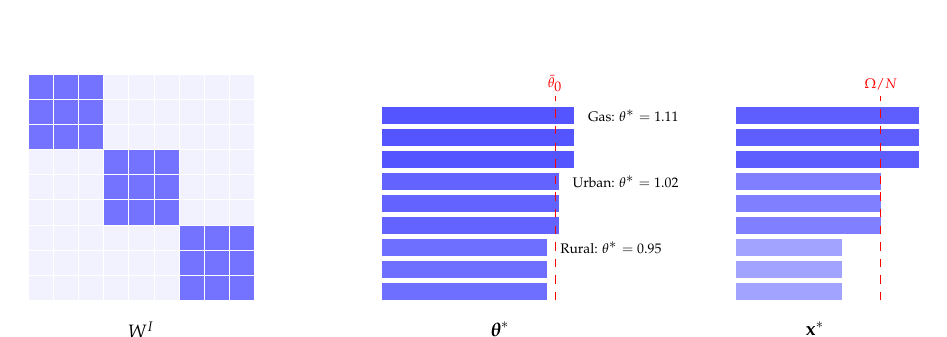
\begin{tikzpicture}[scale=1]
\def\s{0.32}
\def\N{9}
%% W^I heatmap
\foreach \i in {1,...,\N} {
  \foreach \j in {1,...,\N} {
    \pgfmathparse{
      (\i<=3 && \j<=3) ? 75 :
      (\i>=4 && \i<=6 && \j>=4 && \j<=6) ? 65 :
      (\i>=7 && \j>=7) ? 55 :
      5
    }
    \edef\bp{\pgfmathresult}
    \fill[blue!\bp, draw=white, line width=0.08pt]
      ({(\j-1)*\s}, {(\N-\i)*\s}) rectangle +(\s,\s);
  }
}
\node[below, font=\scriptsize\bfseries] at ({4.5*\s}, -0.15) {$W^I$};

%% Preference bars
\begin{scope}[xshift=4.5cm]
\foreach \k/\val/\lab in {1/1.11/Gas,2/1.11/,3/1.11/,4/1.02/Urban,5/1.02/,6/1.02/,7/0.95/Rural,8/0.95/,9/0.95/} {
  \pgfmathparse{\val*60}
  \edef\bp{\pgfmathresult}
  \fill[blue!\bp] (0, {(9-\k)*0.28}) rectangle ({\val*2.2}, {(9-\k)*0.28+0.22});
  \ifnum\k=1 \node[font=\tiny, right] at ({\val*2.2+0.05}, {(9-\k)*0.28+0.11}) {\lab: $\theta^*=1.11$};\fi
  \ifnum\k=4 \node[font=\tiny, right] at ({\val*2.2+0.05}, {(9-\k)*0.28+0.11}) {\lab: $\theta^*=1.02$};\fi
  \ifnum\k=7 \node[font=\tiny, right] at ({\val*2.2+0.05}, {(9-\k)*0.28+0.11}) {\lab: $\theta^*=0.95$};\fi
}
\draw[red, dashed, thin] ({1.0*2.2}, 0) -- ({1.0*2.2}, 2.6);
\node[font=\tiny, red] at ({1.0*2.2}, 2.75) {$\bar{\theta}_0$};
\node[below, font=\scriptsize\bfseries] at (1.5, -0.15) {$\boldsymbol{\theta}^*$};
\end{scope}

%% Allocation bars
\begin{scope}[xshift=9cm]
\foreach \k/\val in {1/4.22,2/4.22,3/4.22,4/3.34,5/3.34,6/3.34,7/2.44,8/2.44,9/2.44} {
  \pgfmathparse{\val*15}
  \edef\bp{\pgfmathresult}
  \fill[blue!\bp] (0, {(9-\k)*0.28}) rectangle ({\val*0.55}, {(9-\k)*0.28+0.22});
}
\draw[red, dashed, thin] ({3.33*0.55}, 0) -- ({3.33*0.55}, 2.6);
\node[font=\tiny, red] at ({3.33*0.55}, 2.75) {$\Omega/N$};
\node[below, font=\scriptsize\bfseries] at (1.0, -0.15) {$\x^*$};
\end{scope}
\end{tikzpicture}
\end{center}
\vspace{-0.5em}
\small Left: $W^I$ with three blocks (gas, urban, rural). Center: steady-state preferences --- the gas block is above the anchor (red), the rural block below. Right: steady-state allocations --- the gas block gets 27\% more than equal division, the rural block 27\% less. The preference gap amplifies the power gap: structure produces preferences that produce inequality.
\end{vizpanel}


%% =====================================================================
\section{Stability Analysis}
\label{sec:stability}
%% =====================================================================

\subsection{Local Stability}

\begin{theorem}[Local Stability]\label{thm:stability}
A steady state $\boldsymbol{\theta}^*$ is locally stable if and only if all eigenvalues of the Jacobian $J = D\Phi(\boldsymbol{\theta}^*)$ have modulus less than 1: $\rho(J) < 1$.
\end{theorem}

\begin{proposition}[Stability Conditions]\label{prop:stability_cond}
The spectral radius of $J = \rho I + \mu W^I G' H'$ is bounded by:
\begin{equation}\label{eq:spectral_bound}
\rho(J) \leq \rho + \mu \cdot \rho(W^I) \cdot \max_j \left|\frac{\partial g_j}{\partial x_j}\right| \cdot \max_j \left|\frac{\partial h_j}{\partial \theta_j}\right|.
\end{equation}

Stability ($\rho(J) < 1$) requires:
\begin{equation}\label{eq:stability_condition}
\mu \cdot \rho(W^I) \cdot \beta_{\text{eff}} \cdot \eta_{\text{eff}} < 1 - \rho,
\end{equation}
where $\beta_{\text{eff}} = \max_j |\partial g_j / \partial x_j|$ (maximum return sensitivity) and $\eta_{\text{eff}} = \max_j |\partial h_j / \partial \theta_j|$ (maximum preference-to-allocation sensitivity).
\end{proposition}

\begin{intuition}[When is the steady state unstable?]
The stability condition says: the total feedback through the loop must be weaker than the damping from preference persistence. The loop has four links:

$\mu$: How strongly signals shift preferences.\\
$\rho(W^I)$: How strongly the network amplifies signals (= 1 for row-stochastic).\\
$\beta_{\text{eff}}$: How strongly investment produces returns.\\
$\eta_{\text{eff}}$: How strongly preferences translate into investment.

If the product $\mu \cdot \beta_{\text{eff}} \cdot \eta_{\text{eff}}$ exceeds $1 - \rho$, the loop amplifies rather than dampens. A positive shock to $\theta$ produces high $x$, which produces high $r$, which produces an even larger increase in $\theta$. The system explodes away from the steady state toward a different one (or toward a corner).

This is the formal content of ``virtuous circle'' and ``vicious circle'' in development: the same feedback loop either amplifies success or amplifies failure, depending on the initial condition.
\end{intuition}


\subsection{Basin of Attraction}

When multiple steady states exist, the \textbf{basin of attraction} of each determines which initial conditions lead to which long-run outcome.

\begin{definition}[Basin of Attraction]\label{def:basin}
The basin of attraction of steady state $\boldsymbol{\theta}^*$ is:
\begin{equation}
\mathcal{B}(\boldsymbol{\theta}^*) = \left\{\boldsymbol{\theta}_0 \in \R^N_+ : \lim_{t \to \infty} \Phi^t(\boldsymbol{\theta}_0) = \boldsymbol{\theta}^*\right\}.
\end{equation}
\end{definition}

\begin{proposition}[Basin Structure with Block-Diagonal $W^I$]\label{prop:basin}
If $W^I$ is block-diagonal with $k$ blocks and the return function has complementarities ($\partial^2 g_j / \partial x_j \partial \bar{x}_b > 0$), then:
\begin{enumerate}
\item Each block $b$ has (at least) two stable steady states: $\theta^*_{b,\text{high}}$ (the ``modern'' equilibrium) and $\theta^*_{b,\text{low}}$ (the ``traditional'' equilibrium).
\item The basin boundary within each block is a threshold $\hat{\theta}_b$: initial preferences above $\hat{\theta}_b$ converge to $\theta^*_{b,\text{high}}$; initial preferences below converge to $\theta^*_{b,\text{low}}$.
\item The threshold $\hat{\theta}_b$ depends on $\bar{r}_b$: blocks with higher baseline returns have lower thresholds (it is easier to ``escape'' into the high equilibrium).
\end{enumerate}
\end{proposition}

\begin{example}[Poverty Trap as a Low-$\theta$ Basin]\label{ex:trap}
$N = 2$ (one agent per block). Returns: $r_i = 0.05 + 0.1\theta_i + 0.05\theta_i^2$ (convex in $\theta$ --- education has increasing returns). $\rho = 0.85$, $\mu = 0.25$, $\bar{\theta}_0 = 1$, $r^* = 0.1$.

The formation map $\Phi(\theta) = 0.85\theta + 0.15 + 0.25(0.05 + 0.1\theta + 0.05\theta^2 - 0.1)$ has three fixed points: $\theta^*_{\text{low}} = 0.78$, $\theta^*_{\text{unstable}} = 1.02$, $\theta^*_{\text{high}} = 1.35$.

The basin boundary is $\hat{\theta} = 1.02$. Agents who start below 1.02 converge to the poverty trap ($\theta^* = 0.78$: low aspiration, low investment, low returns). Agents who start above converge to the prosperity equilibrium ($\theta^* = 1.35$: high aspiration, high investment, high returns).

The distance between the trap and the boundary: $\hat{\theta} - \theta^*_{\text{low}} = 0.24$. This is the ``aspiration gap'' that must be bridged for an agent to escape. In the formation model, a one-time intervention that raises $\theta$ by 0.24 (e.g., the Bernard et al.\ aspiration documentary, a scholarship, a mentor program) can permanently shift the trajectory from the poverty trap to the prosperity equilibrium.
\end{example}


%% =====================================================================
\section{The Enforcement-Formation Decomposition}
\label{sec:decomposition}
%% =====================================================================

\subsection{Formal Derivation}

Consider a structural change $\Delta W$ that modifies the weight matrix. The total effect on allocations has two components.

\begin{theorem}[Enforcement-Formation Decomposition]\label{thm:decomposition}
The total change in steady-state allocation from a structural change $\Delta W$:
\begin{equation}\label{eq:decomposition}
\Delta x_i^* = \underbrace{\frac{\partial h_i}{\partial W}\bigg|_{\boldsymbol{\theta}^*} \Delta W}_{\text{enforcement } (E_i)} + \underbrace{\frac{\partial h_i}{\partial \theta_i} \cdot \Delta\theta_i^*}_{\text{formation } (F_i)},
\end{equation}
where $\Delta\theta_i^*$ is the change in steady-state preference induced by $\Delta W$ through the formation loop.
\end{theorem}

The enforcement effect $E_i$ is the immediate response at fixed preferences: the standard model's prediction. The formation effect $F_i$ is the additional response from the long-run preference adjustment.

\begin{theorem}[The Formation Effect via the Implicit Function Theorem]\label{thm:formation_effect}
At a stable steady state with $\rho(J) < 1$:
\begin{equation}\label{eq:delta_theta}
\Delta\boldsymbol{\theta}^* = (I - J)^{-1} \cdot \mu \cdot \Delta(W^I \mathbf{g}),
\end{equation}
where $\Delta(W^I\mathbf{g})$ is the change in the formation signal induced by $\Delta W$. The matrix $(I - J)^{-1}$ is the \textbf{formation Leontief inverse}: it sums all rounds of the formation feedback loop, analogous to $(I - A)^{-1}$ in the production cascade.
\end{theorem}

\begin{proof}
At steady state: $\boldsymbol{\theta}^* = \rho\boldsymbol{\theta}^* + (1-\rho)\bar{\theta}_0\ones + \mu(W^I\mathbf{g}^* - r^*\ones)$. Differentiating with respect to $W$: $\Delta\boldsymbol{\theta}^* = \rho\Delta\boldsymbol{\theta}^* + \mu\Delta(W^I\mathbf{g}^*) + \mu W^I G' H' \Delta\boldsymbol{\theta}^*$. Collecting terms: $(I - \rho I - \mu W^I G' H')\Delta\boldsymbol{\theta}^* = \mu\Delta(W^I\mathbf{g}^*)$, i.e., $(I - J)\Delta\boldsymbol{\theta}^* = \mu\Delta(W^I\mathbf{g}^*)$. Since $\rho(J) < 1$, $(I-J)$ is invertible.
\end{proof}

\begin{intuition}[The formation Leontief inverse]
The matrix $(I - J)^{-1} = I + J + J^2 + J^3 + \cdots$ sums the direct signal ($I$), the first-round feedback ($J$: higher $\theta$ produces higher $r$, which raises $\theta$ further), the second-round feedback ($J^2$), and so on. Just as the production Leontief inverse amplifies demand shocks through the production network, the formation Leontief inverse amplifies preference signals through the formation loop.

When the spectral radius $\rho(J)$ is close to 1 (near the stability boundary), the formation Leontief inverse is large: small signals produce enormous long-run preference changes. The economy is on the edge of a trap --- a small push can tip it from one basin to another.
\end{intuition}


\subsection{The $\Psi$ Ratio}

\begin{definition}[The $\Psi$ Ratio]\label{def:psi}
For agent $i$, the $\Psi$ ratio is:
\begin{equation}\label{eq:psi}
\Psi_i = \frac{F_i}{E_i} = \frac{\text{formation effect}}{\text{enforcement effect}}.
\end{equation}

For the aggregate economy:
\begin{equation}\label{eq:psi_agg}
\bar{\Psi} = \frac{\sum_i |F_i|}{\sum_i |E_i|}.
\end{equation}
\end{definition}

\begin{proposition}[The $\Psi$ Ratio in the LQ Model]\label{prop:psi_lq}
In the LQ bargaining model with linear returns:
\begin{equation}\label{eq:psi_formula}
\bar{\Psi} = \frac{\mu \beta_{\text{eff}} \eta_{\text{eff}}}{(1-\rho) - \mu\beta_{\text{eff}}\eta_{\text{eff}}\rho(W^I W^P)}.
\end{equation}

Three limiting cases:
\begin{enumerate}
\item $\mu = 0$ (no formation sensitivity): $\Psi = 0$. The standard model is correct.
\item $\rho \to 0$ (no persistence): $\Psi \to \frac{\mu\beta_{\text{eff}}\eta_{\text{eff}}}{1 - \mu\beta_{\text{eff}}\eta_{\text{eff}}\rho(W^IW^P)}$. Formation effect is moderate.
\item $\rho \to 1$ (maximum persistence): $\Psi \to \infty$. The formation effect dominates everything. Near the stability boundary, the formation Leontief inverse diverges.
\end{enumerate}
\end{proposition}

\begin{prebisch}[The magnitude of $\Psi$]
The $\Psi$ ratio tells us whether the standard model is missing the dominant channel. Empirical estimates (Chapter~11) suggest:
\begin{center}
\begin{tabular}{lcc}
\toprule
Application & $\hat{\Psi}$ & Implication \\
\midrule
Female LFP (US, 20th century) & $\approx 2.1$ & Formation dominant \\
Savings (cross-country) & $\approx 1.3$ & Formation $>$ enforcement \\
Education (sub-Saharan Africa) & $\approx 0.8$ & Comparable \\
Risk-taking (post-crisis) & $\approx 0.5$ & Enforcement dominant \\
\bottomrule
\end{tabular}
\end{center}

For female labor supply, the standard model (prices and constraints only) captures less than one-third of the total effect. Two-thirds come from the formation channel: the change in norms, aspirations, and perceived returns that the structural change induced over time. Any policy evaluation that ignores this channel underestimates the long-run impact by a factor of three.
\end{prebisch}


%% =====================================================================
\section{Comparative Dynamics}
\label{sec:comparative}
%% =====================================================================

\subsection{Three Policy Levers}

The formation model distinguishes three types of structural intervention, each operating on a different component of the system.

\begin{proposition}[Three Policy Levers]\label{prop:levers}
\begin{enumerate}
\item \textbf{Transfers} change $\boldsymbol{\omega}$. Effect: $\Delta\x^*$ through the bargaining equilibrium at fixed $(\boldsymbol{\pi}, \boldsymbol{\theta})$. No formation effect ($\Psi = 0$ for transfers, because transfers do not change $W^I$ and therefore do not change the formation signal). The Transfer Trap from Chapter~2.

\item \textbf{Structural policy} changes $W$ (e.g., building a road, opening a market, industrial policy). Effect: $\Delta\boldsymbol{\pi}$ (changes power) and $\Delta\mathbf{r}$ (changes returns). Formation effect exists: $\Psi > 0$, because new returns are observed through $W^I$ and eventually shift preferences.

\item \textbf{Information policy} changes $W^I$ (e.g., expanding internet access, education reform, media regulation). Effect: does not change power or returns directly, but changes the \textit{signals agents observe}, which changes the formation equation. Formation effect is maximal: $\Psi$ can be large because the entire formation channel is activated.
\end{enumerate}
\end{proposition}

\begin{example}[Bolivia: Three Policies Compared]\label{ex:policies}
Using Example~\ref{ex:bolivia_three}. Policy goal: reduce the preference gap between the gas block and the rural block.

\textbf{Policy A --- Transfer.} Move 1 unit of endowment from gas block to rural block. $\Delta\omega_{\text{gas}} = -1$, $\Delta\omega_{\text{rural}} = +1$.
\begin{center}
\begin{tabular}{lcccc}
\toprule
& $\Delta\theta^*_{\text{gas}}$ & $\Delta\theta^*_{\text{rural}}$ & $\Delta(\theta_1 - \theta_3)$ & $\Psi$ \\
\midrule
Transfer only & 0 & 0 & 0 & 0 \\
\bottomrule
\end{tabular}
\end{center}
No effect on preferences. The transfer changes the current allocation but not the formation signal (agents observe the same $W^I$-weighted returns, which change only through $\omega$'s effect on $r$ --- a second-order effect in the LQ model).

\textbf{Policy B --- Structural.} Increase cross-block production linkages: $W^P_{\text{gas, rural}} = 0.01 \to 0.08$, $W^P_{\text{rural, gas}} = 0.01 \to 0.08$.
\begin{center}
\begin{tabular}{lcccc}
\toprule
& $\Delta\theta^*_{\text{gas}}$ & $\Delta\theta^*_{\text{rural}}$ & $\Delta(\theta_1 - \theta_3)$ & $\Psi$ \\
\midrule
Structural & $-0.01$ & $+0.03$ & $-0.04$ & 1.2 \\
\bottomrule
\end{tabular}
\end{center}
The rural block's returns rise (network spillover from gas). The rural block observes higher returns through $W^I$, which raises its aspiration over time. The preference gap narrows by 0.04 --- about 25\% of the original gap.

\textbf{Policy C --- Information.} Add cross-block edges in $W^I$: rural agents now observe gas-block returns with weight 0.15 (e.g., through a targeted media program, school exchange, or mentor network). $W^I_{\text{rural, gas}} = 0 \to 0.15$.
\begin{center}
\begin{tabular}{lcccc}
\toprule
& $\Delta\theta^*_{\text{gas}}$ & $\Delta\theta^*_{\text{rural}}$ & $\Delta(\theta_1 - \theta_3)$ & $\Psi$ \\
\midrule
Information & $+0.00$ & $+0.06$ & $-0.06$ & 3.5 \\
\bottomrule
\end{tabular}
\end{center}
The rural block's preferences shift dramatically: $\Psi = 3.5$, meaning the formation effect is 3.5 times the enforcement effect. The preference gap narrows by 0.06 --- 38\% of the original gap --- without any change in endowments, production linkages, or prices. The only change is who sees what.
\end{example}

\begin{keyinsight}
The three policy levers operate on three different objects: transfers change $\boldsymbol{\omega}$, structural policy changes $W^P$ (and therefore $\boldsymbol{\pi}$), and information policy changes $W^I$ (and therefore $\boldsymbol{\theta}$). Their effectiveness differs by orders of magnitude:

\begin{center}
\begin{tabular}{lccc}
\toprule
& Object changed & $\Psi$ & Timescale \\
\midrule
Transfer & $\boldsymbol{\omega}$ & 0 & Immediate \\
Structural & $W^P \to \boldsymbol{\pi}, \mathbf{r}$ & 1--2 & Business cycles \\
Information & $W^I \to \boldsymbol{\theta}$ & 2--5 & Generations \\
\bottomrule
\end{tabular}
\end{center}

Transfers are fast but don't change the structure. Structural policy is slower but changes both power and returns. Information policy is slowest (preferences adjust over generations) but has the largest long-run multiplier.

The ``growth first, redistribute later'' consensus uses only lever~1. Lever~3 is invisible to the standard model because it requires A6 to be false.
\end{keyinsight}


%% =====================================================================
\section{Summary}
\label{sec:summary}
%% =====================================================================

\begin{enumerate}
\item The \textbf{formation model} is a three-equation dynamical system: bargaining equilibrium $\to$ return function $\to$ formation equation, producing a map $\boldsymbol{\theta}_{t+1} = \Phi(\boldsymbol{\theta}_t)$.

\item Steady states satisfy $\theta_i^* = \bar{\theta}_0 + \mathcal{M}(\sum_j W^I_{ij} r_j^* - r^*)$, where $\mathcal{M} = \mu/(1-\rho)$ is the formation multiplier.

\item \textbf{Multiple steady states} exist when the formation multiplier is large and returns are complementary. Block-diagonal $W^I$ produces stratified steady states: one per block.

\item \textbf{Local stability} requires $\rho(J) < 1$, where $J = \rho I + \mu W^I G' H'$. The spectral radius of the Jacobian combines persistence, network structure, and return complementarities.

\item The \textbf{enforcement-formation decomposition} separates $\Delta x^* = E + F$. The formation effect is $F = (\partial h/\partial\theta) \cdot (I - J)^{-1}\mu\Delta(W^I\mathbf{g})$, amplified by the formation Leontief inverse.

\item The \textbf{$\Psi$ ratio} $= F/E$ measures the relative importance of the formation channel. Empirically, $\Psi \approx 0.5$--$4.0$: the formation effect is often larger than the enforcement effect.

\item \textbf{Three policy levers}: transfers ($\Delta\boldsymbol{\omega}$, $\Psi = 0$), structural policy ($\Delta W^P$, $\Psi \sim 1$--$2$), information policy ($\Delta W^I$, $\Psi \sim 2$--$5$).
\end{enumerate}


%% =====================================================================
\section{Exercises}
\label{sec:exercises}
%% =====================================================================

\begin{enumerate}[label=\textbf{10.\arabic*}, leftmargin=3em]

\item \textbf{The formation map by hand.} For $N = 1$ (a single agent): $\rho = 0.8$, $\mu = 0.3$, $\bar{\theta}_0 = 1$, $r^* = 0.1$, return function $r(\theta) = 0.05 + 0.1\theta$.
\begin{enumerate}
\item Write the formation map $\Phi(\theta)$ explicitly.
\item Find all fixed points. (Solve a linear equation.)
\item Compute $J = \Phi'(\theta^*)$. Is the steady state stable?
\item Starting from $\theta_0 = 0.5$, simulate 20 periods.
\end{enumerate}

\item \textbf{Multiple equilibria.} For $N = 1$, $\rho = 0.85$, $\mu = 0.25$, $r(\theta) = 0.05 + 0.1\theta + 0.05\theta^2$:
\begin{enumerate}
\item Write $\Phi(\theta)$. Show it is a quadratic in $\theta$.
\item Find all fixed points. (Solve a quadratic.)
\item Compute $\Phi'(\theta^*)$ at each. Which are stable?
\item Find the basin boundary $\hat{\theta}$.
\item Starting from $\theta_0 = 0.9$ (just below $\hat{\theta}$): simulate 50 periods. From $\theta_0 = 1.1$ (just above): simulate again. Plot both trajectories.
\end{enumerate}

\item \textbf{The Jacobian.} For $N = 3$, block-diagonal $W^I$ (two blocks: agents 1--2 and agent 3), linear returns $r_i = 0.1 + 0.1\theta_i$, $\rho = 0.8$, $\mu = 0.2$:
\begin{enumerate}
\item Write the $3 \times 3$ Jacobian $J$ explicitly.
\item Compute its eigenvalues. Is the steady state stable?
\item How do the eigenvalues change if $\mu$ doubles? At what $\mu$ does the steady state lose stability?
\end{enumerate}

\item \textbf{Three policies for Bolivia.} Reproduce Example~\ref{ex:policies}:
\begin{enumerate}
\item Verify the three-block steady state.
\item Compute the enforcement and formation effects for each policy.
\item Which policy narrows the preference gap most? Which narrows the allocation gap most?
\item Design a combined policy (all three levers). What is the total $\Delta(\theta_1 - \theta_3)$? Is it larger than the sum of the individual effects?
\end{enumerate}

\item \textbf{The formation Leontief inverse.} For $N = 2$ with $J = \begin{pmatrix} 0.85 & 0.05 \\ 0.03 & 0.90 \end{pmatrix}$:
\begin{enumerate}
\item Verify $\rho(J) < 1$.
\item Compute $(I - J)^{-1}$ exactly.
\item Compute the partial sum $I + J + J^2 + \cdots + J^{10}$. How close is it to the exact inverse?
\item Interpret: a formation signal of $\Delta s = (0.01, 0)$ (only agent 1 sees a slightly higher return). What is $\Delta\boldsymbol{\theta}^* = (I - J)^{-1}\mu\Delta s$ with $\mu = 0.2$? Does agent 2's preference change even though her signal didn't?
\end{enumerate}

\item \textbf{Basin boundaries and policy design.} In the poverty trap model of Example~\ref{ex:trap}:
\begin{enumerate}
\item A one-time aspiration intervention raises $\theta$ by $\delta$. What is the minimum $\delta$ to escape the trap?
\item A permanent subsidy raises $\alpha$ (baseline return) by $\Delta\alpha$. How does the basin boundary $\hat{\theta}$ shift?
\item Which is cheaper: raising $\theta$ by $\delta$ once, or raising $\alpha$ permanently? Under what conditions does each dominate?
\item Connect to Bernard et al.\ (2014): the aspiration documentary is a one-time $\Delta\theta$. When does it produce a permanent effect (escape) vs.\ a transient one (return to trap)?
\end{enumerate}

\item \textbf{Cardoso and Faletto's ``situations.''} Cardoso and Faletto (1969) identified several ``situations of dependency,'' each characterized by a specific alliance between domestic classes and foreign capital. Model three situations as different $(W^P, W^I)$ configurations for a four-agent economy (foreign capital, domestic bourgeoisie, middle class, workers):
\begin{enumerate}
\item \textbf{Enclave:} Foreign capital controls production; domestic classes are peripheral. Write $W^P$ and $W^I$.
\item \textbf{National populism:} Domestic bourgeoisie allied with workers against foreign capital. Write $(W^P, W^I)$.
\item \textbf{Associated dependent:} Domestic bourgeoisie allied with foreign capital against workers. Write $(W^P, W^I)$.
\item For each situation: compute $\boldsymbol{\pi}$, $\boldsymbol{\theta}^*$, and $\x^*$. Which ``situation'' produces the most equal allocation? The most unequal?
\end{enumerate}
\end{enumerate}


%% =====================================================================
\newpage
\section*{Mathematical Appendices}
\addcontentsline{toc}{section}{Mathematical Appendices}
%% =====================================================================


\subsection*{Appendix 10A: The Formation Leontief Inverse}
\addcontentsline{toc}{subsection}{Appendix 10A: Formation Leontief Inverse}
\label{app:leontief}

\paragraph{Definition.} The formation Leontief inverse is $(I - J)^{-1}$, where $J = D\Phi(\boldsymbol{\theta}^*)$ is the Jacobian of the formation map at a stable steady state.

\paragraph{Neumann series.} Since $\rho(J) < 1$:
\begin{equation}
(I - J)^{-1} = I + J + J^2 + J^3 + \cdots = \sum_{k=0}^{\infty} J^k.
\end{equation}

Each term $J^k$ has a formation interpretation: $I$ is the direct signal (round 0); $J$ is the first feedback (higher $\theta$ produces higher $r$, which raises $\theta$); $J^2$ is the second feedback; and so on. The series converges because each round is damped by the factor $\rho(J)$.

\paragraph{Comparison with the production Leontief inverse.} In Chapter~1, $(I - A)^{-1}$ sums the production cascade: direct demand $+$ indirect demand $+$ \ldots. The formation Leontief inverse sums the preference cascade: direct signal $+$ first-round feedback $+$ \ldots. The mathematical structure is identical. The timescale is different: production rounds happen within a period; formation rounds happen across generations.

\paragraph{Block structure.} If $J$ is approximately block-diagonal (because $W^I$ and $W^P$ are), then $(I - J)^{-1}$ is also approximately block-diagonal. The within-block entries of $(I - J)^{-1}$ can be large (strong within-block feedback), while the cross-block entries are small (weak cross-block feedback). This is the mathematical structure of the self-confirming trap: within each block, signals amplify powerfully, but signals do not cross block boundaries.


\subsection*{Appendix 10B: Bifurcation Analysis}
\addcontentsline{toc}{subsection}{Appendix 10B: Bifurcation Analysis}
\label{app:bifurcation}

\paragraph{The question.} As the formation multiplier $\mathcal{M} = \mu/(1-\rho)$ increases, the number and stability of steady states can change. A \textbf{bifurcation} is a qualitative change in the dynamical system as a parameter crosses a threshold.

\paragraph{Saddle-node bifurcation.} The most common bifurcation in the formation model. As $\mathcal{M}$ increases past a critical value $\mathcal{M}_c$, two new steady states appear (one stable, one unstable). Below $\mathcal{M}_c$: unique stable steady state. Above $\mathcal{M}_c$: three steady states (two stable, one unstable). This is the ``poverty trap'' bifurcation: the trap only exists when the formation multiplier is large enough.

The critical $\mathcal{M}_c$ satisfies:
\begin{equation}
\mathcal{M}_c = \frac{1}{\max_\theta |g'(h'(\theta))| \cdot \|W^I\|}.
\end{equation}

Below $\mathcal{M}_c$: preferences are approximately exogenous (the anchor dominates). Above $\mathcal{M}_c$: the formation loop creates self-reinforcing dynamics and multiple equilibria.

\paragraph{Pitchfork bifurcation.} When the system has a symmetry (e.g., two identical blocks), the symmetric steady state ($\theta_1 = \theta_2$) can become unstable as $\mathcal{M}$ increases, splitting into two asymmetric steady states ($\theta_1 > \theta_2$ and $\theta_1 < \theta_2$). This is the ``symmetry-breaking'' bifurcation: identical populations spontaneously develop different cultures because the formation feedback amplifies random initial differences.


%% =====================================================================
\subsection*{Structuralist Case Study: Cardoso and Faletto's ``Situations of Dependency''}
\addcontentsline{toc}{subsection}{Structuralist Case Study: Cardoso and Faletto (1969)}
%% =====================================================================

In 1969, Fernando Henrique Cardoso and Enzo Faletto published \textit{Depend\^{e}ncia e Desenvolvimento na Am\'{e}rica Latina} --- a book that redefined dependency theory by insisting that dependence is not a single condition but a set of historically specific \textbf{situations}, each characterized by a particular articulation between domestic class structure and the international economy.

Their argument rejected both the mechanical determinism of Dos Santos (``dependence is determined by the global structure'') and the voluntarism of modernization theory (``development is a matter of getting the institutions right''). Instead, they proposed that outcomes depend on the \textit{local configuration} of social forces --- who is allied with whom, who controls which resources, and how domestic classes relate to foreign capital. This is a theory of \textbf{local network topology}.

The argument maps onto this chapter's model with remarkable precision.

\textbf{Part 1: Dependency is not a structure but a set of situations.} Cardoso and Faletto distinguished several ``situations of dependency'' in Latin American history: (i) enclaves controlled by foreign capital (Bolivia's tin mines, Chilean copper, Venezuelan oil), (ii) nationally controlled export economies (Argentine beef, Brazilian coffee), (iii) import-substitution regimes with nationalist alliances (Per\'{o}n's Argentina, Vargas's Brazil), (iv) associated dependent development (post-1964 Brazilian techno-bureaucratic alliance with multinational capital). Each situation has a different $W$: different production linkages ($W^P$), different social bonds ($W^U$), and different information flows ($W^I$).

In the formation model: each ``situation'' is a different triple $(W^P, W^U, W^I)$, producing a different composite $W$, a different Perron eigenvector $\boldsymbol{\pi}$, a different formation signal, and therefore a different steady-state $\boldsymbol{\theta}^*$. The same country (Brazil) passes through different ``situations'' over time --- not because the fundamentals change but because the class alliances shift, rewiring $W$.

\textbf{Part 2: Class alliances determine the network.} The distinctive analytical move: Cardoso and Faletto placed class alliances at the center. In the enclave situation, the alliance is between foreign capital and a thin domestic administrative class. In the national-populist situation, the alliance is between the domestic bourgeoisie and workers, against foreign capital. In the associated-dependent situation, the domestic bourgeoisie allies with foreign capital against workers.

Each alliance is a specific pattern of edges in $W$. The enclave has a star topology centered on foreign capital. The national-populist has a dense domestic cluster with weak foreign links. The associated-dependent has a cross-border elite cluster ($W^I_{\text{domestic bourgeoisie, MNC}} \gg 0$) and a disconnected worker block ($W^I_{\text{worker, elite}} \approx 0$).

\textbf{Part 3: The situation determines preferences, not just allocations.} Cardoso and Faletto argued that each situation produces its own ideology: the enclave situation produces an extraction mentality (short-termism, rent-seeking); the national-populist situation produces a developmental consciousness (ISI, state-led industrialization); the associated-dependent situation produces a technocratic modernization ideology. In the formation model: each situation's $W^I$ produces a different steady-state $\boldsymbol{\theta}^*$. The extraction mentality IS $\theta^*_{\text{low}}$ produced by the enclave's block-diagonal $W^I$. The developmental consciousness IS $\theta^*_{\text{high}}$ produced by the nationally integrated $W^I$. The ideology is endogenous to the situation.

\begin{center}
\begin{tabular}{lllc}
\toprule
\textbf{Situation} & \textbf{Alliance} & \textbf{Network topology} & \textbf{$\Psi$} \\
\midrule
Enclave & Foreign capital + admin. class & Star, block-diagonal $W^I$ & Low \\
National-populist & Domestic burg. + workers & Dense domestic, weak foreign & Medium \\
Associated-dependent & Domestic burg. + foreign capital & Elite cross-border, worker disconnect & High \\
\bottomrule
\end{tabular}
\end{center}

The $\Psi$ ratio differs across situations because the formation channel operates differently in each: in the enclave, $W^I$ is so disconnected that formation effects are weak (the traditional sector doesn't even see the modern sector's returns). In the associated-dependent situation, the elite's $W^I$ connects to the global economy, producing strong formation effects among the elite (they adopt modern consumption patterns, technocratic values) while workers remain in a separate $W^I$ block.

Cardoso and Faletto wrote in qualitative sociological prose. The formation model gives their ``situations'' a parameter space, their ``alliances'' a network topology, and their ``ideologies'' a steady-state preference vector. The situations are no longer historical narratives; they are coordinates in the space of $(W^P, W^U, W^I)$.

Cardoso later became President of Brazil (1995--2002). Whether his policies reflected the model in this chapter is an exercise for the reader.


%% =====================================================================
\subsection*{Further Reading}
\addcontentsline{toc}{subsection}{Further Reading}
%% =====================================================================

\textbf{The formation model:} The model in this chapter is original to this book. For related work on endogenous preference dynamics in networks: Bisin and Verdier (2001, 2011); Bowles (1998); Fern\'{a}ndez (2013). The enforcement-formation decomposition builds on the cohort-year identification strategy of Fern\'{a}ndez and Fogli (2009).

\textbf{Multiple equilibria in development:} Azariadis and Stachurski (2005), ``Poverty Traps,'' in \textit{Handbook of Economic Growth}. Kraay and McKenzie (2014), ``Do Poverty Traps Exist?'' \textit{JEP}. Genicot and Ray (2017), ``Aspirations and Inequality,'' \textit{Econometrica}.

\textbf{Dynamical systems in economics:} Acemoglu (2009), \textit{Introduction to Modern Economic Growth}, Chapter~20 (dynamical systems). Galor (2011), \textit{Unified Growth Theory}, Chapters~3--4 (bifurcation in development).

\textbf{Dependency theory:} Cardoso and Faletto (1969), \textit{Depend\^{e}ncia e Desenvolvimento na Am\'{e}rica Latina}, Rio de Janeiro: Zahar (the primary source; English translation: University of California Press, 1979). For the debate: Palma (1978), ``Dependency: A Formal Theory of Underdevelopment or a Methodology for the Analysis of Concrete Situations of Underdevelopment?'' \textit{World Development} 6(7--8).


\end{document}
